\documentclass[11pt,letterpaper]{article}

\usepackage[spanish,es-tabla,es-nodecimaldot]{babel}
\usepackage{fontspec}
\usepackage{amsmath,amssymb,mathtools}
\usepackage[margin=2.3cm]{geometry}
\usepackage{graphicx}
\usepackage{booktabs}
\usepackage{siunitx}
\usepackage{xcolor}
\usepackage{listings}
\usepackage{caption}
\usepackage[most]{tcolorbox}
\usepackage{hyperref}

\sisetup{output-decimal-marker={.}, per-mode=symbol, separate-uncertainty}
\hypersetup{colorlinks=true, linkcolor=blue!50!black, citecolor=blue!50!black, urlcolor=blue!50!black}
\captionsetup{font=small, labelfont=bf}
\setlength{\parskip}{0.45em}
\setlength{\parindent}{0pt}

\definecolor{codebg}{RGB}{248,248,248}
\lstset{
  language=Matlab, basicstyle=\ttfamily\footnotesize, backgroundcolor=\color{codebg},
  keywordstyle=\color{blue!70!black}\bfseries, commentstyle=\color{green!40!black}\itshape,
  stringstyle=\color{red!60!black}, frame=single, rulecolor=\color{black!25},
  breaklines=true, columns=fullflexible, keepspaces=true, showstringspaces=false,
  numbers=left, numberstyle=\tiny\color{black!50}, xleftmargin=1.5em
}

\newtcolorbox{idea}[1][]{colback=blue!4, colframe=blue!45!black, fonttitle=\bfseries, title={#1}}
\newtcolorbox{resultado}[1][]{colback=green!4, colframe=green!40!black, fonttitle=\bfseries, title={#1}}
\newtcolorbox{cuidado}[1][]{colback=orange!6, colframe=orange!70!black, fonttitle=\bfseries, title={#1}}

\newcommand{\VT}{V_T}
\newcommand{\dd}{\,\mathrm{d}}

\title{\textbf{Tarea 1 — Óptica No Lineal}\\[0.3em]
\large Puntos 2 y 3: espectro de salida de sistemas no lineales\\ y validez de la aproximación de Taylor}
\author{Juan Esteban Rodríguez Ochoa\\ \small Escuela de Física, Universidad Nacional de Colombia — Medellín, 2026-II}
\date{27 de septiembre de 2026}

\begin{document}
\maketitle

\begin{abstract}
\noindent Se calcula, analíticamente y con MATLAB, la amplitud del espectro de Fourier de la salida de
dos sistemas no lineales sin memoria: un dispositivo de ley cuadrática $i=v^2$ excitado con dos
tonos (50 y \SI{120}{Hz}) y un diodo, $i=i_0[\exp(v/\VT)-1]$, polarizado en \SI{0.3}{V} con una
señal de \SI{0.2}{V} a \SI{50}{Hz}. Para el primero la solución exacta es un número finito de líneas
(DC, armónicos, suma y diferencia de frecuencias); para el segundo la solución exacta se expresa con
funciones de Bessel modificadas $I_n(x)$ y contiene infinitos armónicos. En el punto 3 se estima la
razón entre el segundo y tercer armónico del diodo con la serie de Taylor truncada en orden 3,
obteniéndose $6\VT/V_1=0.78$ frente al valor exacto $I_2(x)/I_3(x)=1.4065$, y se explica por qué la
aproximación falla: el parámetro de expansión $x=V_1/\VT\approx7.7$ no es pequeño. Todas las
predicciones analíticas coinciden con la FFT numérica hasta la sexta cifra.
\end{abstract}

\tableofcontents
\newpage

%=====================================================================
\section{Enunciados y plan de trabajo}
%=====================================================================

\textbf{Punto 2.} \emph{Use Matlab para dibujar la amplitud de la transformada de Fourier de la salida
versus frecuencia de los siguientes sistemas y entradas:}
\begin{enumerate}
  \item[(a)] Dispositivo con la ley $i=v^2$ con entrada $v=\cos(2\pi 50t)+\cos(2\pi 120t)$.
  \item[(b)] Un diodo mezclador con función de transferencia $i=i_0\left[\exp(ev/kT)-1\right]$, donde
  $i_0=\SI{10}{pA}$ es la corriente de polarización inversa, $kT/e=\SI{26}{mV}$ a temperatura
  ambiente. La entrada es $v=0.3+0.2\cos(2\pi 50t)$, en voltios.
\end{enumerate}

\textbf{Punto 3.} \emph{En el problema 2b, estimar la relación de la amplitud entre el segundo y tercer
armónico, considerando el término cuadrado y cúbico en la expansión de serie de Taylor de la función de
transferencia. Compare con los resultados obtenidos en 2b.}

\begin{idea}[Estrategia general]
Para cada caso se sigue el mismo camino:
\begin{enumerate}
  \item \textbf{Predecir analíticamente} qué frecuencias aparecen en la salida y con qué amplitud.
  \item \textbf{Calcular numéricamente} el espectro con la FFT de MATLAB.
  \item \textbf{Comparar} ambos resultados. Si coinciden, tanto el código como el análisis son
  confiables; si no, uno de los dos tiene un error.
\end{enumerate}
Hacer primero la predicción analítica es lo que convierte una gráfica en un resultado verificado.
\end{idea}

\textbf{Notación.} En todo el documento $j=\sqrt{-1}$, para no confundir la unidad imaginaria con la
corriente $i(t)$. Se usa $\omega=2\pi f$ y $\theta=\omega t$. Las amplitudes del espectro se reportan
como \emph{amplitudes de coseno}: si una componente es $A\cos(2\pi f t+\varphi)$, su amplitud es $A$.

%=====================================================================
\section{Herramientas matemáticas}
%=====================================================================

\subsection{¿Por qué un sistema no lineal crea frecuencias nuevas?}

Un sistema \emph{lineal} solo puede cambiar la amplitud y la fase de cada frecuencia de entrada: si
entra $\cos\omega t$, sale $A\cos(\omega t+\varphi)$. Un sistema \emph{no lineal sin memoria} aplica una
función $g$ al valor instantáneo de la entrada, $i(t)=g(v(t))$. Si $g$ contiene potencias $v^n$, al elevar
un coseno a una potencia aparecen cosenos de frecuencias múltiplos (y, si hay varias frecuencias,
combinaciones de ellas). Esa es exactamente la física de la óptica no lineal: la polarización de un
material se expande como \cite[ec.~(1.1.2), p.~2]{boyd}
\begin{equation}
  \tilde P(t)=\epsilon_0\left[\chi^{(1)}\tilde E(t)+\chi^{(2)}\tilde E^2(t)+\chi^{(3)}\tilde E^3(t)+\cdots\right],
  \label{eq:boyd}
\end{equation}
y los términos $\tilde E^2$ y $\tilde E^3$ generan el segundo y tercer armónico, la suma y diferencia de
frecuencias, etc. En este taller el ``campo'' es el voltaje $v$ y la ``polarización'' es la corriente $i$.

\subsection{Identidades trigonométricas que se usarán}

Todas se deducen de la fórmula de Euler, $\cos\alpha=\tfrac12(e^{j\alpha}+e^{-j\alpha})$:
\begin{align}
  \cos^2\alpha &= \tfrac12\left(1+\cos 2\alpha\right), \label{eq:cos2}\\
  \cos^3\alpha &= \tfrac14\left(3\cos\alpha+\cos 3\alpha\right), \label{eq:cos3}\\
  \cos\alpha\cos\beta &= \tfrac12\left[\cos(\alpha-\beta)+\cos(\alpha+\beta)\right]. \label{eq:prod}
\end{align}
Por ejemplo, para \eqref{eq:cos3}:
$\cos^3\alpha=\tfrac18(e^{j\alpha}+e^{-j\alpha})^3=\tfrac18\left(e^{3j\alpha}+3e^{j\alpha}+3e^{-j\alpha}+e^{-3j\alpha}\right)
=\tfrac14\cos3\alpha+\tfrac34\cos\alpha$. Esta misma identidad aparece en Boyd para la generación de tercer
armónico \cite[ec.~(1.2.13), p.~11]{boyd}.

\subsection{Espectro de amplitud de una señal periódica}

La transformada de Fourier de una señal se define aquí como
\begin{equation}
  X(f)=\int_{-\infty}^{\infty}x(t)\,e^{-j2\pi f t}\dd t .
\end{equation}
Para un coseno, $x(t)=A\cos(2\pi f_0 t)$, se obtiene
\begin{equation}
  X(f)=\frac{A}{2}\left[\delta(f-f_0)+\delta(f+f_0)\right],
\end{equation}
es decir, dos deltas de peso $A/2$ en $\pm f_0$. Toda la información está en las frecuencias positivas
si se juntan ambas mitades: el \textbf{espectro de amplitud unilateral} asigna la amplitud $A$ a la
frecuencia $f_0$, y a la componente DC (constante $A_0$) la amplitud $A_0$. Por eso, cuando la salida se
pueda escribir como $i(t)=A_0+\sum_k A_k\cos(2\pi f_k t+\varphi_k)$, \emph{la gráfica pedida consiste en líneas
verticales de altura $A_k$ en las frecuencias $f_k$}.

\begin{cuidado}[Convención de signo]
Boyd escribe los campos como $E e^{-j\omega t}+\text{c.c.}$ y MATLAB usa $e^{-j2\pi f t}$ en la transformada
directa. El signo del exponente solo cambia la fase del espectro, no su módulo; la amplitud
$|X(f)|$ que se pide es la misma en cualquier convención.
\end{cuidado}

\subsection{De la transformada continua a la FFT}\label{sec:fft}

MATLAB no calcula integrales sino la \textbf{transformada discreta de Fourier} (DFT) de $N$ muestras
$x[n]=x(n/f_s)$, tomadas con frecuencia de muestreo $f_s$ durante un tiempo $T=N/f_s$:
\begin{equation}
  X[k]=\sum_{n=0}^{N-1}x[n]\,e^{-j2\pi kn/N},\qquad k=0,1,\dots,N-1 .
\end{equation}
El índice $k$ corresponde a la frecuencia $f_k=k\,f_s/N=k/T$; la separación entre bins es
$\Delta f=1/T$. La función \texttt{fft} calcula esta suma eficientemente.

\textbf{Normalización.} Supongamos $x[n]=A\cos(2\pi k_0 n/N)$ con $k_0$ entero. Usando Euler,
\begin{equation}
  X[k]=\frac{A}{2}\sum_{n=0}^{N-1}\left[e^{-j2\pi(k-k_0)n/N}+e^{-j2\pi(k+k_0)n/N}\right].
\end{equation}
La suma geométrica $\sum_{n=0}^{N-1}e^{-j2\pi m n/N}$ vale $N$ si $m$ es múltiplo de $N$ y $0$ en cualquier
otro caso. Entonces $X[k_0]=AN/2$ y $X[N-k_0]=AN/2$ (la ``frecuencia negativa''), y todos los demás bins
son exactamente cero. Por tanto:
\begin{equation}
  \boxed{\;A_k=\frac{2\,|X[k]|}{N}\ \ (k\ge1),\qquad A_0=\frac{|X[0]|}{N}\;}
\end{equation}
El factor 2 junta las dos mitades del espectro; la componente DC no tiene pareja y no lo lleva.

\textbf{Elección de parámetros.} Se usó $f_s=\SI{10}{kHz}$ y $T=\SI{1}{s}$ ($N=10\,000$):
\begin{itemize}
  \item \emph{Nyquist:} la frecuencia más alta con amplitud apreciable es \SI{240}{Hz} en (a) y del
  orden de \SI{600}{Hz} en (b); $f_s/2=\SI{5}{kHz}$ está muy por encima, así que no hay aliasing.
  \item \emph{Sin fuga espectral:} con $T=\SI{1}{s}$ todas las frecuencias involucradas (múltiplos de
  \SI{10}{Hz}) completan un número entero de ciclos, de modo que caen exactamente en un bin
  ($\Delta f=\SI{1}{Hz}$) y la suma geométrica anterior es exacta. Si $T$ no fuera un número entero de
  periodos, cada línea se ``derramaría'' sobre los bins vecinos (\emph{leakage}) y su altura disminuiría.
  \item El vector de tiempo es \texttt{t = (0:N-1)/fs}, \emph{sin} incluir $t=T$: la DFT supone que la señal
  se repite con periodo $T$, y repetir la muestra final duplicaría un punto.
\end{itemize}

%=====================================================================
\section{Punto 2a: dispositivo de ley cuadrática}
%=====================================================================

\subsection{Planteamiento}
\begin{equation}
  i(t)=v^2(t),\qquad v(t)=\cos\alpha+\cos\beta,\qquad \alpha=2\pi f_1 t,\ \beta=2\pi f_2 t,
\end{equation}
con $f_1=\SI{50}{Hz}$ y $f_2=\SI{120}{Hz}$. El enunciado no da un coeficiente, así que se toma
$i=k v^2$ con $k=\SI{1}{A/V^2}$; con otro $k$ todo el espectro simplemente se escala.

\subsection{Derivación analítica paso a paso}

\textbf{Paso 1 — desarrollar el cuadrado.}
\begin{equation}
  i=(\cos\alpha+\cos\beta)^2=\cos^2\alpha+2\cos\alpha\cos\beta+\cos^2\beta .
\end{equation}

\textbf{Paso 2 — linealizar cada término} con \eqref{eq:cos2} y \eqref{eq:prod}:
\begin{align}
  \cos^2\alpha &= \tfrac12+\tfrac12\cos2\alpha, \\
  2\cos\alpha\cos\beta &= \cos(\beta-\alpha)+\cos(\alpha+\beta), \\
  \cos^2\beta &= \tfrac12+\tfrac12\cos2\beta .
\end{align}

\textbf{Paso 3 — sumar y reemplazar las frecuencias.}
\begin{equation}
  \boxed{\,i(t)=1+\cos(2\pi\,70\,t)+\tfrac12\cos(2\pi\,100\,t)+\cos(2\pi\,170\,t)+\tfrac12\cos(2\pi\,240\,t)\,}
  \label{eq:2a}
\end{equation}
Esto es \emph{exacto}: al ser $g(v)=v^2$ un polinomio de grado 2, la salida tiene un número finito de líneas.

\subsection{Interpretación: los mismos procesos que en óptica no lineal}

Si en Boyd se toma $\tilde E(t)=E_1e^{-j\omega_1t}+E_2e^{-j\omega_2t}+\text{c.c.}$ y se calcula
$\tilde P^{(2)}=\epsilon_0\chi^{(2)}\tilde E^2$, aparecen términos en $2\omega_1$, $2\omega_2$,
$\omega_1+\omega_2$, $\omega_1-\omega_2$ y frecuencia cero \cite[ecs.~(1.2.3)--(1.2.5), p.~6]{boyd}.
Es exactamente el mismo cálculo que acabamos de hacer:

\begin{table}[h]
\centering
\caption{Componentes de la salida del dispositivo cuadrático y su proceso óptico análogo.}
\label{tab:2a}
\begin{tabular}{@{}cccl@{}}
\toprule
Frecuencia & Origen & Amplitud (A) & Proceso análogo en óptica no lineal \\
\midrule
\SI{0}{Hz}   & $\tfrac12+\tfrac12$         & 1   & Rectificación óptica (OR) \\
\SI{70}{Hz}  & $f_2-f_1$                   & 1   & Generación de diferencia de frecuencias (DFG) \\
\SI{100}{Hz} & $2f_1$                      & 0.5 & Generación de segundo armónico (SHG) \\
\SI{170}{Hz} & $f_1+f_2$                   & 1   & Generación de suma de frecuencias (SFG) \\
\SI{240}{Hz} & $2f_2$                      & 0.5 & Generación de segundo armónico (SHG) \\
\bottomrule
\end{tabular}
\end{table}

Observaciones:
\begin{itemize}
  \item \textbf{Las frecuencias de entrada (50 y \SI{120}{Hz}) no aparecen en la salida.} El término
  cuadrático solo produce sumas y diferencias de \emph{pares} de frecuencias; para reproducir la entrada
  haría falta un término lineal.
  \item \textbf{Los productos cruzados pesan el doble que los armónicos} (1 frente a 0.5), por el factor
  2 de $2\cos\alpha\cos\beta$. Lo mismo ocurre en Boyd, donde SFG y DFG llevan $2\chi^{(2)}E_1E_2$ y SHG lleva
  $\chi^{(2)}E_1^2$.
  \item La salida es periódica con periodo $1/\gcd(50,120)=\SI{0.1}{s}$ (\SI{10}{Hz} es el máximo común
  divisor), por lo que $T=\SI{1}{s}$ contiene exactamente 10 periodos.
\end{itemize}

\subsection{Implementación en MATLAB}

Las líneas esenciales de \texttt{punto2a.m} (código completo en el apéndice~\ref{app:codigo}):
\begin{lstlisting}[numbers=none]
fs = 10e3;  T = 1;  N = round(fs*T);  t = (0:N-1)/fs;
v = cos(2*pi*50*t) + cos(2*pi*120*t);   % entrada (V)
i = v.^2;                               % salida (A)
X = fft(i)/N;                           % DFT normalizada
f = (0:N/2)*fs/N;                       % eje de frecuencias positivas (Hz)
A = abs(X(1:N/2+1));  A(2:end-1) = 2*A(2:end-1);  % espectro unilateral
stem(f, A)                              % grafica |I(f)| vs f
\end{lstlisting}

\subsection{Resultados}

\begin{figure}[h]
\centering
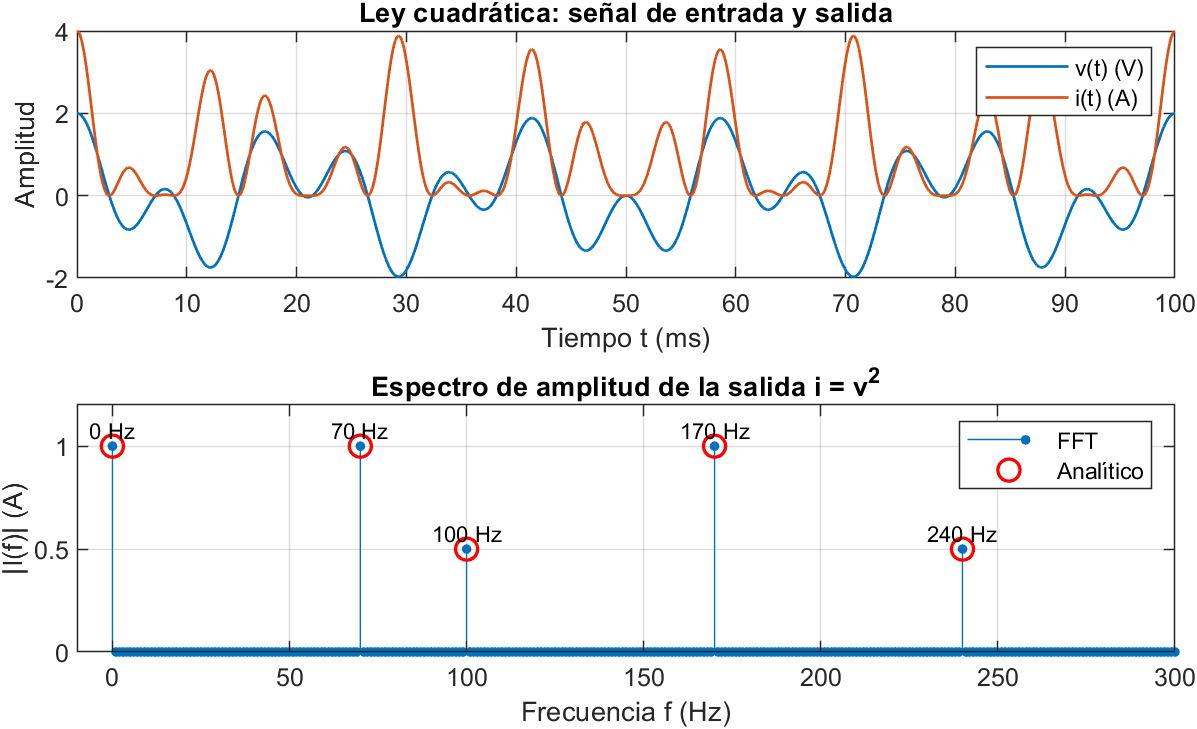
\includegraphics[width=0.92\textwidth]{figuras/punto2a_espectro.png}
\caption{Punto 2a. Arriba: entrada $v(t)$ y salida $i(t)=v^2$ en los primeros \SI{100}{ms} (un periodo de la
salida). Abajo: amplitud del espectro de la salida calculada con la FFT (puntos azules) y predicción
analítica de la ec.~\eqref{eq:2a} (círculos rojos).}
\label{fig:2a}
\end{figure}

\begin{table}[h]
\centering
\caption{Punto 2a: amplitudes obtenidas por FFT frente a la predicción analítica.}
\begin{tabular}{@{}ccc@{}}
\toprule
$f$ (Hz) & $|I|$ FFT (A) & $|I|$ analítico (A) \\
\midrule
0 & 1.000000 & 1 \\ 70 & 1.000000 & 1 \\ 100 & 0.500000 & 0.5 \\ 170 & 1.000000 & 1 \\ 240 & 0.500000 & 0.5 \\
\bottomrule
\end{tabular}
\end{table}

\textbf{Verificación independiente (teorema de Parseval).} La potencia media de la señal debe ser igual a
la suma de las potencias de sus componentes: $\langle i^2\rangle=A_0^2+\tfrac12\sum_{k\ge1}A_k^2
=1+\tfrac12(1+1+0.25+0.25)=2.25$. El promedio numérico de $i^2(t)$ en MATLAB da exactamente $2.250000$.

%=====================================================================
\section{Punto 2b: diodo mezclador}
%=====================================================================

\subsection{El modelo del diodo}

La ecuación de Shockley del diodo es
\begin{equation}
  i=i_0\left[\exp\!\left(\frac{ev}{kT}\right)-1\right]=i_0\left[e^{v/\VT}-1\right],\qquad \VT\equiv\frac{kT}{e}=\SI{26}{mV}.
\end{equation}
$\VT$ es el \emph{voltaje térmico}: la escala de voltaje sobre la cual la exponencial cambia apreciablemente.
Cada vez que $v$ aumenta en $\VT$, la corriente se multiplica por $e\approx2.72$. La entrada es
$v(t)=V_0+V_1\cos\omega t$ con $V_0=\SI{0.3}{V}$ (polarización DC), $V_1=\SI{0.2}{V}$ y $f=\SI{50}{Hz}$.

\subsection{Paso 1: separar la polarización}

Como $e^{a+b}=e^ae^b$,
\begin{equation}
  i(t)=i_0\,e^{V_0/\VT}\,e^{(V_1/\VT)\cos\omega t}-i_0
      \;=\;I_s\,e^{x\cos\omega t}-i_0,
\end{equation}
donde se definieron dos cantidades clave:
\begin{align}
  I_s &\equiv i_0\,e^{V_0/\VT}=(\SI{10}{pA})\,e^{11.538}=(\SI{10}{pA})(1.0259\times10^5)=\SI{1.0259}{\micro A},\\
  x &\equiv \frac{V_1}{\VT}=\frac{\SI{0.2}{V}}{\SI{0.026}{V}}=7.6923 .
\end{align}
$I_s$ es la corriente en el punto de operación y $x$ mide \emph{qué tan grande es la señal comparada con la
escala de la no linealidad}. Este número controla todo el problema.

\subsection{Paso 2: serie de Fourier de $e^{x\cos\theta}$ — funciones de Bessel modificadas}

La función $e^{x\cos\theta}$ es periódica en $\theta$ con periodo $2\pi$ y par, así que tiene una serie de
Fourier de solo cosenos. Sus coeficientes se obtienen con la \textbf{función generatriz de las funciones de
Bessel modificadas}. Se parte de
\begin{equation}
  \exp\!\left[\frac{x}{2}\left(t+\frac1t\right)\right]=e^{xt/2}\,e^{x/(2t)}
  =\left(\sum_{m=0}^{\infty}\frac{(x/2)^m t^m}{m!}\right)\left(\sum_{k=0}^{\infty}\frac{(x/2)^k t^{-k}}{k!}\right).
\end{equation}
Agrupando las potencias $t^n$ (es decir, $m=n+k$):
\begin{equation}
  \exp\!\left[\frac{x}{2}\left(t+\frac1t\right)\right]=\sum_{n=-\infty}^{\infty}I_n(x)\,t^n,
  \qquad I_n(x)=\sum_{k=0}^{\infty}\frac{(x/2)^{2k+n}}{k!\,(k+n)!},
  \label{eq:Inserie}
\end{equation}
que es la definición en serie de la función de Bessel modificada de primera especie, $I_n(x)$, con
$I_{-n}=I_n$ para $n$ entero. Ahora se toma $t=e^{j\theta}$, de modo que $\tfrac12(t+1/t)=\cos\theta$:
\begin{equation}
  e^{x\cos\theta}=\sum_{n=-\infty}^{\infty}I_n(x)e^{jn\theta}
  =I_0(x)+\sum_{n=1}^{\infty}I_n(x)\left(e^{jn\theta}+e^{-jn\theta}\right)
  =I_0(x)+2\sum_{n=1}^{\infty}I_n(x)\cos n\theta .
  \label{eq:jacobi}
\end{equation}
(Equivalentemente, los coeficientes de Fourier son $I_n(x)=\frac1\pi\int_0^\pi e^{x\cos\theta}\cos n\theta\dd\theta$.)

\subsection{Paso 3: la salida exacta y su espectro}

Sustituyendo \eqref{eq:jacobi} con $\theta=\omega t$:
\begin{equation}
  \boxed{\,i(t)=\underbrace{\left[I_sI_0(x)-i_0\right]}_{\text{DC}}+\sum_{n=1}^{\infty}\underbrace{2I_sI_n(x)}_{A_n}\cos(2\pi\,n\,50\,t)\,}
  \label{eq:2b}
\end{equation}
La salida contiene DC y \textbf{todos} los armónicos de \SI{50}{Hz} (100, 150, 200, \ldots\,Hz), con amplitud
$A_n=2I_sI_n(x)$. En MATLAB, $I_n(x)$ se evalúa con \texttt{besseli(n,x)}.

\begin{table}[h]
\centering
\caption{Punto 2b: valores de $I_n(x)$ para $x=7.6923$ y amplitudes de la corriente. La columna FFT es el
resultado numérico de \texttt{punto2b.m}.}
\label{tab:2b}
\begin{tabular}{@{}cccccc@{}}
\toprule
$n$ & $f$ (Hz) & $I_n(x)$ & $|I|$ Bessel (mA) & $|I|$ FFT (mA) & Relativa al fundamental \\
\midrule
0 & 0   & 320.778 & 0.329075 & 0.329075 & 0.536 \\
1 & 50  & 299.136 & 0.613746 & 0.613746 & 1.000 \\
2 & 100 & 243.003 & 0.498576 & 0.498576 & 0.812 \\
3 & 150 & 172.775 & 0.354487 & 0.354487 & 0.578 \\
4 & 200 & 108.239 & 0.222076 & 0.222076 & 0.362 \\
5 & 250 & 60.207  & 0.123528 & 0.123528 & 0.201 \\
6 & 300 & 29.970  & 0.061490 & 0.061490 & 0.100 \\
7 & 350 & 13.453  & 0.027603 & 0.027603 & 0.045 \\
8 & 400 & 5.485   & 0.011254 & 0.011254 & 0.018 \\
9 & 450 & 2.044   & 0.004195 & 0.004195 & 0.007 \\
10 & 500 & 0.701  & 0.001438 & 0.001438 & 0.002 \\
\bottomrule
\end{tabular}
\end{table}

Ejemplo de cálculo para el fundamental: $A_1=2(\SI{1.0259}{\micro A})(299.136)=\SI{0.6137}{mA}$. Para DC:
$A_0=(\SI{1.0259}{\micro A})(320.778)-\SI{10}{pA}=\SI{0.3291}{mA}$ (el término $-i_0$ es despreciable).

\subsection{¿Por qué hay tantos armónicos? Forma de la corriente}

\begin{figure}[h]
\centering
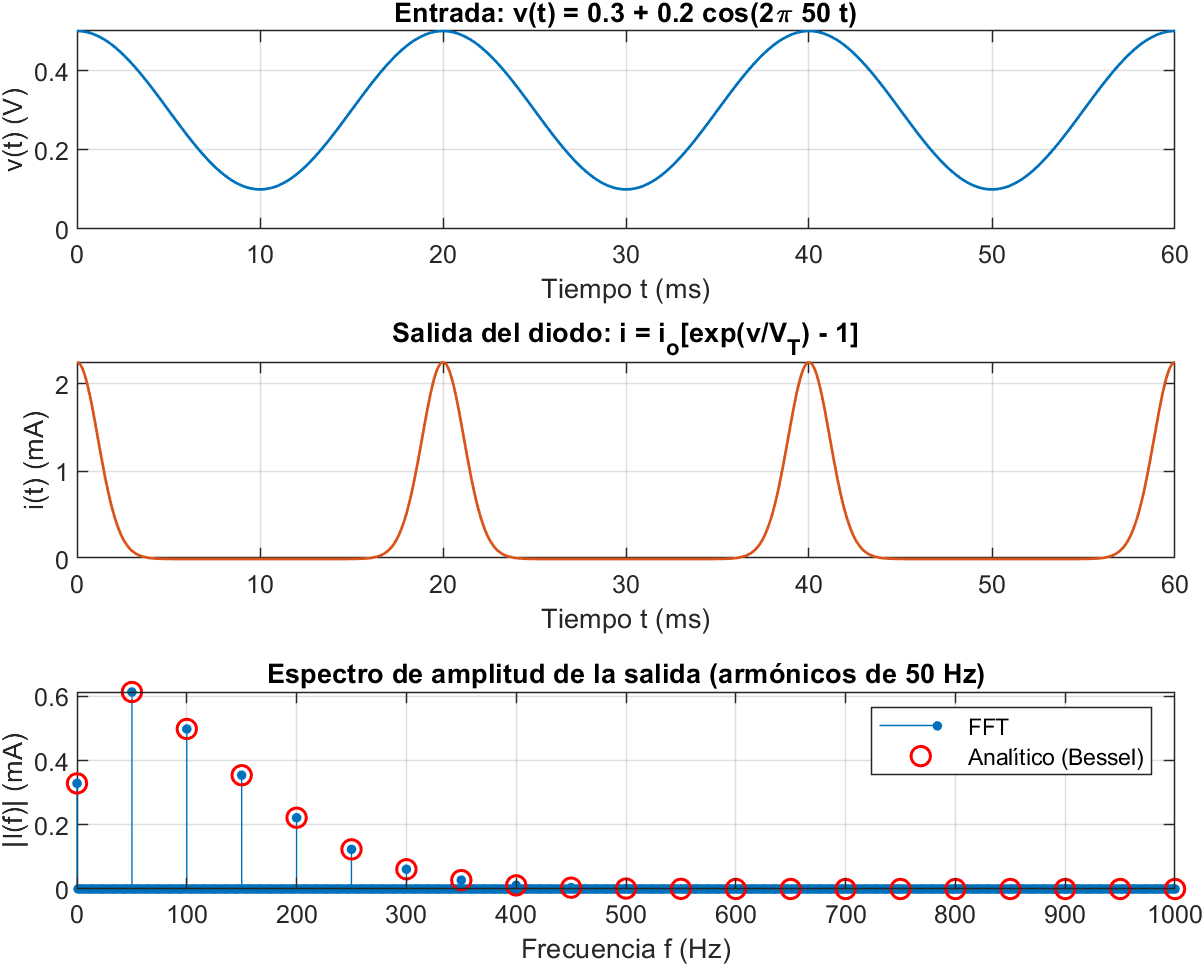
\includegraphics[width=0.92\textwidth]{figuras/punto2b_espectro.png}
\caption{Punto 2b. Arriba: voltaje de entrada. Centro: corriente del diodo; es un tren de pulsos estrechos
de \SI{2.25}{mA} de pico, uno por ciclo. Abajo: amplitud del espectro (FFT en azul, ec.~\eqref{eq:2b} en rojo).}
\label{fig:2b}
\end{figure}

La corriente (fig.~\ref{fig:2b}, centro) no se parece a la entrada: es casi cero durante la mayor parte del
ciclo y tiene un pico agudo cuando $v$ es máximo. La razón es que $v$ recorre de \SI{0.1}{V} a \SI{0.5}{V},
es decir, $2V_1/\VT\approx15$ ``escalas térmicas'', y la corriente cambia en un factor $e^{15.4}\approx5\times10^6$
entre el mínimo y el máximo. Un pulso estrecho en el tiempo tiene un espectro ancho en frecuencia.

Esto se puede cuantificar. Cerca del máximo, $\cos\theta\approx1-\theta^2/2$, así que
$e^{x\cos\theta}\approx e^x e^{-x\theta^2/2}$: un pulso gaussiano de ancho angular $1/\sqrt x$, es decir
$\sigma_t=1/(\omega\sqrt x)\approx\SI{1.1}{ms}$. Su espectro también es gaussiano, y para $x$ grande
\begin{equation}
  \frac{I_n(x)}{I_0(x)}\approx e^{-n^2/(2x)},
\end{equation}
de modo que el número de armónicos relevantes es del orden de $\sqrt{x}\approx3$; los armónicos decaen
lentamente al principio y luego muy rápido (fig.~\ref{fig:2blog}). Por ejemplo, esta aproximación da
$I_3/I_0\approx e^{-9/15.38}=0.56$, frente al valor exacto $172.775/320.778=0.54$.

\begin{figure}[h]
\centering
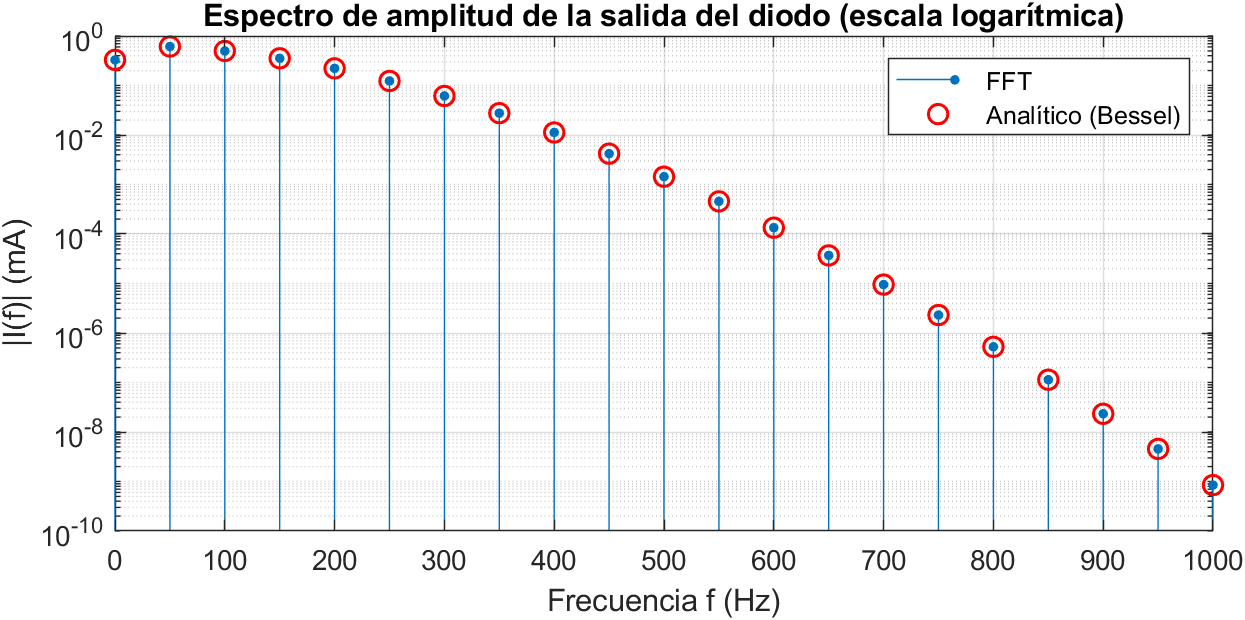
\includegraphics[width=0.92\textwidth]{figuras/punto2b_espectro_log.png}
\caption{Punto 2b en escala logarítmica. La FFT sigue a la solución de Bessel a lo largo de 9 órdenes de magnitud;
el decaimiento de los armónicos altos es más rápido que exponencial.}
\label{fig:2blog}
\end{figure}

\subsection{Implementación en MATLAB}

\begin{lstlisting}[numbers=none]
io = 10e-12;  VT = 26e-3;  V0 = 0.3;  V1 = 0.2;
v = V0 + V1*cos(2*pi*50*t);              % entrada (V)
i = io*(exp(v/VT) - 1);                  % salida (A)
% ... misma FFT y normalizacion que en 2a ...
x = V1/VT;  n = 0:20;                    % prediccion analitica
A_an = 2*io*exp(V0/VT)*besseli(n, x);
A_an(1) = io*(exp(V0/VT)*besseli(0, x) - 1);  % DC
\end{lstlisting}

\subsection{Verificaciones}

Además de la coincidencia línea por línea de la tabla~\ref{tab:2b}, hay tres comprobaciones independientes:
\begin{enumerate}
  \item \textbf{DC = valor medio.} El promedio temporal de $i(t)$ calculado directamente es
  \SI{0.329075}{mA}, igual a $A_0$.
  \item \textbf{Suma de amplitudes = corriente pico.} En $t=0$ todos los cosenos valen 1, así que
  $i(0)=\sum_n A_n$. La suma de las amplitudes hasta $n=12$ da \SI{2.248058}{mA}, y
  $i(0)=I_se^{x}-i_0=\SI{2.248107}{mA}$; la diferencia es el aporte de los armónicos $n>12$.
  \item \textbf{Parseval.} El valor RMS de $i(t)$ calculado en el tiempo y a partir de las amplitudes
  espectrales coincide: \SI{0.719990}{mA} en ambos casos.
\end{enumerate}

\begin{cuidado}[¿Por qué ``mezclador'' si solo hay armónicos?]
Con una sola frecuencia de entrada, lo único que puede producir la no linealidad son armónicos de esa
frecuencia (más DC). Un diodo funciona como \emph{mezclador} cuando recibe dos tonos $f_1$ y $f_2$ (por ejemplo
señal y oscilador local): entonces la exponencial genera todas las combinaciones $mf_1\pm nf_2$, incluida la
frecuencia intermedia $|f_1-f_2|$, igual que en el punto 2a pero con infinitos órdenes.
\end{cuidado}

%=====================================================================
\section{Punto 3: razón entre segundo y tercer armónico por serie de Taylor}
%=====================================================================

\subsection{Idea}

La serie de Taylor de la función de transferencia es el análogo exacto de la expansión
\eqref{eq:boyd} de la polarización. En ella, \emph{el segundo armónico viene del término cuadrático y el
tercer armónico del término cúbico}. El punto 3 pide quedarse solo con esos términos, estimar la razón
$A_2/A_3$ y compararla con el resultado exacto de 2b.

\subsection{Paso 1: ¿alrededor de qué punto se expande?}

La señal oscila alrededor de la polarización $V_0$, así que lo natural es expandir alrededor del
\textbf{punto de operación}. Se define la parte variable de la entrada,
\begin{equation}
  u(t)=v(t)-V_0=V_1\cos\omega t,
\end{equation}
y, como en el punto 2b,
\begin{equation}
  i=I_s\,e^{u/\VT}-i_0 .
\end{equation}
(En la sección~\ref{sec:v0} se muestra qué ocurre si se expande alrededor de $v=0$.)

\subsection{Paso 2: serie de Taylor hasta orden 3}

\begin{equation}
  e^{u/\VT}=1+\frac{u}{\VT}+\frac{1}{2!}\left(\frac{u}{\VT}\right)^2+\frac{1}{3!}\left(\frac{u}{\VT}\right)^3+\mathcal{O}\!\left(\frac{u^4}{\VT^4}\right).
\end{equation}
Con $u/\VT=x\cos\omega t$:
\begin{equation}
  i\approx I_s\left[1+x\cos\omega t+\frac{x^2}{2}\cos^2\omega t+\frac{x^3}{6}\cos^3\omega t\right]-i_0 .
\end{equation}

\subsection{Paso 3: linealizar las potencias}

Usando \eqref{eq:cos2} y \eqref{eq:cos3}:
\begin{align}
  \frac{x^2}{2}\cos^2\omega t &= \frac{x^2}{4}+\frac{x^2}{4}\cos2\omega t,\\
  \frac{x^3}{6}\cos^3\omega t &= \frac{x^3}{8}\cos\omega t+\frac{x^3}{24}\cos3\omega t .
\end{align}

\subsection{Paso 4: agrupar por frecuencia}

\begin{equation}
  i\approx\underbrace{I_s\left(1+\frac{x^2}{4}\right)-i_0}_{\text{DC}}
  +\underbrace{I_s\left(x+\frac{x^3}{8}\right)}_{f}\cos\omega t
  +\underbrace{I_s\frac{x^2}{4}}_{2f}\cos2\omega t
  +\underbrace{I_s\frac{x^3}{24}}_{3f}\cos3\omega t .
\end{equation}
El segundo armónico sale \emph{solo} del término cuadrático y el tercero \emph{solo} del cúbico.

\subsection{Paso 5: la razón}

\begin{equation}
  \boxed{\;\frac{A_{2f}}{A_{3f}}\approx\frac{I_sx^2/4}{I_sx^3/24}=\frac{6}{x}=\frac{6\VT}{V_1}
  =\frac{6\,(\SI{0.026}{V})}{\SI{0.2}{V}}=0.78\;}
\end{equation}
Nótese que $I_s$ (y por tanto $i_0$ y $V_0$) se cancela: la razón solo depende de $V_1/\VT$.

\subsection{Comparación con el resultado exacto de 2b}

Del punto 2b, $A_n=2I_sI_n(x)$, así que la razón exacta es
\begin{equation}
  \left.\frac{A_{2f}}{A_{3f}}\right|_{\text{exacta}}=\frac{I_2(x)}{I_3(x)}=\frac{243.003}{172.775}=1.4065,
\end{equation}
que coincide con la razón medida en la FFT (1.4065).

\begin{table}[h]
\centering
\caption{Taylor hasta orden 3 (alrededor de $V_0$) frente al resultado exacto, para $V_1=\SI{0.2}{V}$.}
\label{tab:3}
\begin{tabular}{@{}lccc@{}}
\toprule
Magnitud & Taylor (orden 3) & Exacto (Bessel/FFT) & Taylor/Exacto \\
\midrule
DC (mA)             & 0.0162 & 0.3291 & 0.049 \\
\SI{50}{Hz} (mA)    & 0.0663 & 0.6137 & 0.108 \\
\SI{100}{Hz} (mA)   & 0.0152 & 0.4986 & 0.030 \\
\SI{150}{Hz} (mA)   & 0.0195 & 0.3545 & 0.055 \\
\midrule
\textbf{Razón $A_{2f}/A_{3f}$} & \textbf{0.780} & \textbf{1.4065} & \textbf{0.555} (error $-44.5$\,\%) \\
\bottomrule
\end{tabular}
\end{table}

\begin{resultado}[Resultado del punto 3]
La serie de Taylor truncada en orden 3 predice $A_{2f}/A_{3f}=6\VT/V_1=0.78$, mientras que el valor exacto
(punto 2b) es $1.4065$: la estimación \textbf{subestima la razón en un 44.5\,\%}, y las amplitudes absolutas
quedan entre 10 y 30 veces por debajo de las reales. La aproximación \textbf{no es válida} para estas
condiciones porque $x=V_1/\VT\approx7.7$ no es pequeño.
\end{resultado}

\subsection{¿Por qué falla la aproximación?}

\textbf{1. La serie truncada no representa a la exponencial.} La serie de Taylor de $e^x$ converge para
todo $x$, pero necesita \emph{muchos} términos cuando $x$ es grande. Truncada en orden 3,
\begin{equation}
  1+x+\frac{x^2}{2}+\frac{x^3}{6}\bigg|_{x=7.69}=114.1
  \qquad\text{frente a}\qquad e^{7.69}=2191.4 .
\end{equation}
Los términos de orden 4, 5, 6, \ldots\ (que se despreciaron) son en realidad mayores que los retenidos: el
término general $x^n/n!$ crece mientras $n<x$, y alcanza su máximo cerca de $n\approx7$. Además, esos
términos de orden superior también contribuyen a $2f$ y $3f$: por ejemplo, $\cos^4$ contiene $\cos2\theta$ y
$\cos^5$ contiene $\cos3\theta$.

\textbf{2. Por qué la razón falla ``menos'' que las amplitudes.} El error de truncamiento afecta a ambos
armónicos en la misma dirección (ambos se subestiman mucho), y al dividir se cancela parcialmente.

\textbf{3. Taylor es el límite de señal pequeña del resultado exacto.} Para $x\ll1$ basta el primer
término de la serie \eqref{eq:Inserie}, $I_n(x)\approx(x/2)^n/n!$, y entonces
\begin{equation}
  \frac{I_2(x)}{I_3(x)}\approx\frac{(x/2)^2/2!}{(x/2)^3/3!}=\frac{x^2/8}{x^3/48}=\frac{6}{x},
\end{equation}
exactamente el resultado de Taylor. Incluyendo la siguiente corrección de \eqref{eq:Inserie} se obtiene
$I_2/I_3\approx(6/x)(1+x^2/48)$, que muestra cuándo empieza a fallar: la corrección es del
10\,\% cuando $x\approx2$. En el extremo opuesto, $x\gg1$, la aproximación gaussiana de la sección
anterior da $I_2/I_3\approx e^{(9-4)/(2x)}\to1$, en lugar de $6/x\to0$.

\begin{figure}[h]
\centering
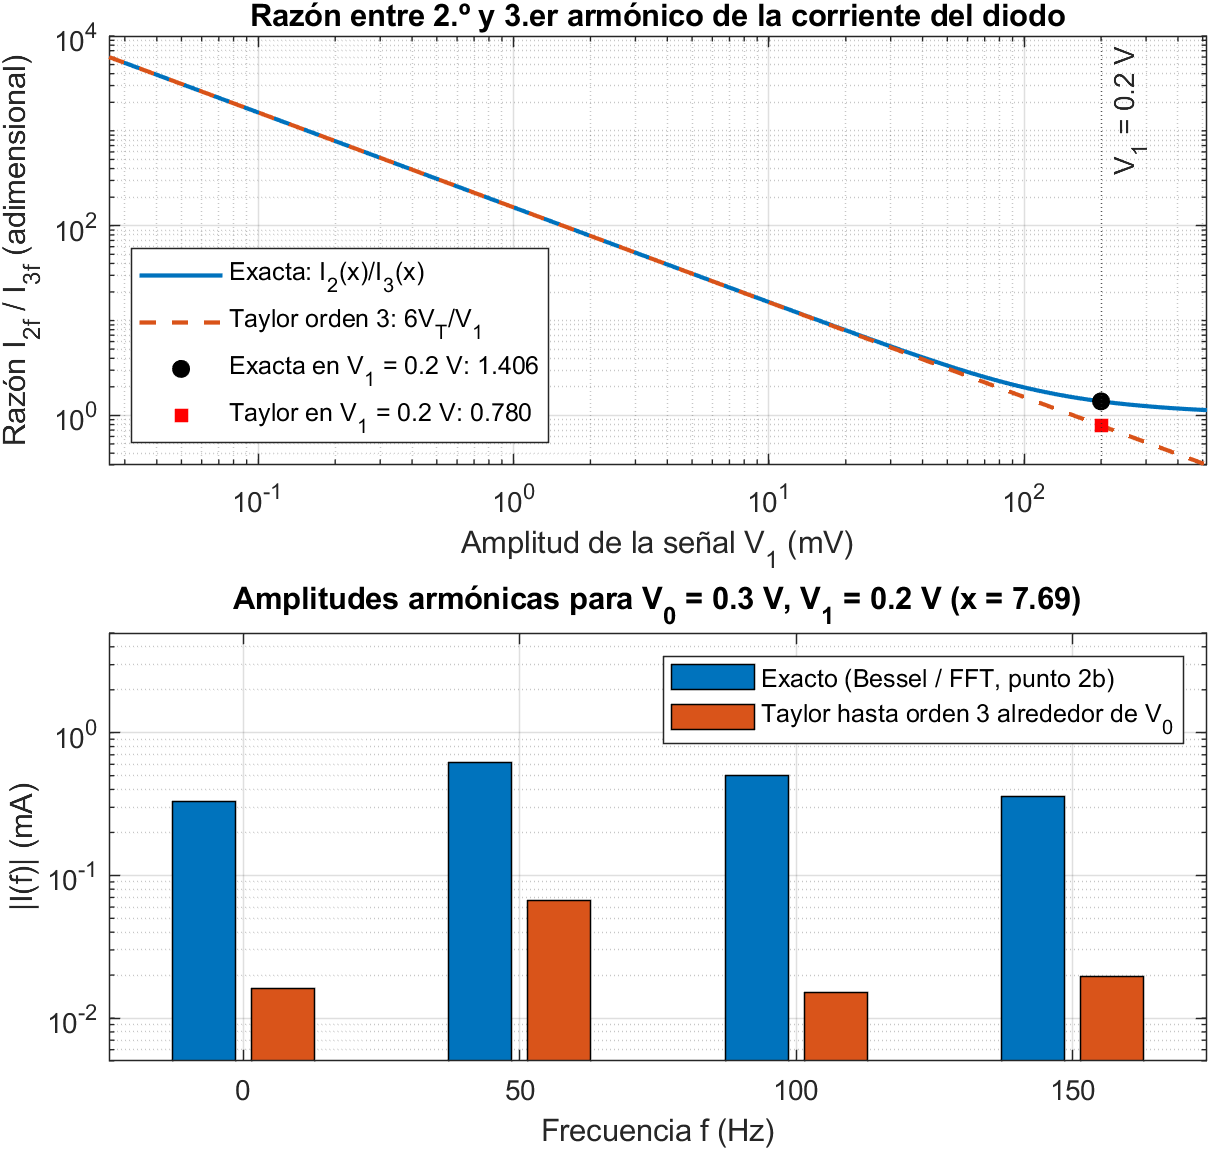
\includegraphics[width=0.9\textwidth]{figuras/punto3_taylor_vs_exacto.png}
\caption{Punto 3. Arriba: razón $A_{2f}/A_{3f}$ en función de la amplitud de la señal $V_1$; la curva exacta
$I_2(x)/I_3(x)$ (azul) y la de Taylor $6\VT/V_1$ (rojo, discontinua) coinciden para señales pequeñas y se
separan cuando $V_1$ se acerca a unas decenas de mV. Abajo: amplitudes de DC y de los tres primeros
armónicos para $V_1=\SI{0.2}{V}$ (escala logarítmica).}
\label{fig:3}
\end{figure}

\textbf{4. Rango de validez.} Numéricamente (fig.~\ref{fig:3}), la estimación $6/x$ tiene un error menor
al 10\,\% solo si $x<2.4$, es decir, $V_1<\SI{63}{mV}\approx2.4\,\VT$. Con $V_1=\SI{0.2}{V}$ se está muy
fuera de ese rango.

\subsection{Variante: expansión alrededor de $v=0$}\label{sec:v0}

Si se expande directamente $e^{v/\VT}$ alrededor de $v=0$,
\begin{equation}
  i\approx i_0\left[\frac{v}{\VT}+\frac{v^2}{2\VT^2}+\frac{v^3}{6\VT^3}\right],\qquad v=V_0+V_1\cos\omega t,
\end{equation}
hay que desarrollar las potencias de $v$ completas:
\begin{align}
  v^2 &= V_0^2+2V_0V_1\cos\omega t+V_1^2\cos^2\omega t,\\
  v^3 &= V_0^3+3V_0^2V_1\cos\omega t+3V_0V_1^2\cos^2\omega t+V_1^3\cos^3\omega t .
\end{align}
Ahora el término cúbico también aporta al segundo armónico (vía $3V_0V_1^2\cos^2\omega t$):
\begin{align}
  A_{2f} &= i_0\left[\frac{V_1^2}{4\VT^2}+\frac{3V_0V_1^2}{2\cdot6\VT^3}\right]=\frac{i_0V_1^2}{4\VT^2}\left(1+\frac{V_0}{\VT}\right),\\
  A_{3f} &= i_0\,\frac{V_1^3}{4\cdot6\VT^3}=\frac{i_0V_1^3}{24\VT^3},
\end{align}
\begin{equation}
  \frac{A_{2f}}{A_{3f}}=\frac{6(\VT+V_0)}{V_1}=\frac{6(\SI{0.326}{V})}{\SI{0.2}{V}}=9.78 .
\end{equation}
Esta estimación es mucho peor (casi 7 veces el valor exacto) y las amplitudes que predice son del orden de
nA en lugar de mA. El motivo: el voltaje llega hasta \SI{0.5}{V}, es decir $v/\VT\approx19$ unidades
lejos del centro de la expansión. \emph{Conclusión práctica: una serie de potencias debe centrarse en el
punto de operación del sistema}, y aun así solo es útil si la excursión alrededor de él es pequeña
comparada con la escala de la no linealidad.

\subsection{Conexión con la óptica no lineal}

La expansión \eqref{eq:boyd} es también una serie de potencias, y su validez depende de lo mismo: que el
campo aplicado sea pequeño frente a la escala característica de la no linealidad. En un material, esa
escala es el campo atómico, $E_{\text{at}}=e/(4\pi\epsilon_0a_0^2)\approx\SI{5.14e11}{V/m}$, y cada orden
superior está suprimido aproximadamente por un factor $E/E_{\text{at}}$ (de ahí la estimación
$\chi^{(2)}\sim\chi^{(1)}/E_{\text{at}}$) \cite[p.~3]{boyd}. En el diodo, la escala es $\VT$ y cada orden
está suprimido por $V_1/\VT$:

\begin{table}[h]
\centering
\caption{Analogía entre el diodo y un medio óptico no lineal.}
\begin{tabular}{@{}lll@{}}
\toprule
& Diodo & Medio óptico \\
\midrule
Entrada & $v(t)$ & $\tilde E(t)$ \\
Respuesta & $i(t)$ & $\tilde P(t)$ \\
Escala de la no linealidad & $\VT=\SI{26}{mV}$ & $E_{\text{at}}\approx\SI{5e11}{V/m}$ \\
Parámetro de expansión & $V_1/\VT$ & $E/E_{\text{at}}$ \\
Segundo armónico viene de & término $u^2$ & $\chi^{(2)}\tilde E^2$ \\
Tercer armónico viene de & término $u^3$ & $\chi^{(3)}\tilde E^3$ \\
\bottomrule
\end{tabular}
\end{table}

En óptica, incluso con láseres intensos, $E/E_{\text{at}}\ll1$, por eso la expansión perturbativa en
$\chi^{(n)}$ funciona muy bien y los efectos de orden alto son cada vez más débiles. En el diodo del
problema, en cambio, $V_1/\VT\approx7.7$: estamos en el régimen ``no perturbativo'', donde truncar la serie
no tiene sentido y hay que usar la solución exacta.

%=====================================================================
\section{Conclusiones}
%=====================================================================

\begin{enumerate}
  \item \textbf{Punto 2a.} La ley cuadrática produce exactamente cinco líneas: DC (\SI{1}{A}),
  $f_2-f_1=\SI{70}{Hz}$ (\SI{1}{A}), $2f_1=\SI{100}{Hz}$ (\SI{0.5}{A}), $f_1+f_2=\SI{170}{Hz}$
  (\SI{1}{A}) y $2f_2=\SI{240}{Hz}$ (\SI{0.5}{A}). Son los análogos de la rectificación óptica, DFG, SHG y SFG
  producidos por $\chi^{(2)}$. Las frecuencias de entrada no aparecen en la salida.
  \item \textbf{Punto 2b.} El diodo produce DC y todos los armónicos de \SI{50}{Hz}, con amplitudes exactas
  $A_n=2i_0e^{V_0/\VT}I_n(V_1/\VT)$. Como $V_1/\VT\approx7.7$, la corriente es un tren de pulsos estrechos y
  los armónicos son fuertes hasta $n\approx6$ (\SI{300}{Hz}).
  \item \textbf{Punto 3.} Taylor hasta orden 3 alrededor de $V_0$ da $A_{2f}/A_{3f}=6\VT/V_1=0.78$ frente al
  valor exacto $1.4065$ (error del $-44.5$\,\%). La aproximación solo es válida (error $<10$\,\%) para
  $V_1\lesssim\SI{63}{mV}$. Expandir alrededor de $v=0$ es aún peor ($9.78$).
  \item \textbf{Método.} En los tres casos la FFT de MATLAB reproduce la solución analítica hasta la sexta
  cifra significativa, gracias a muestrear un número entero de periodos (sin fuga espectral) y a normalizar
  el espectro unilateral con $2|X[k]|/N$.
\end{enumerate}

\begin{thebibliography}{9}
\bibitem{boyd} R. W. Boyd, \emph{Nonlinear Optics}, 3.ª ed., Academic Press, 2008. Cap.~1:
§1.1 (ec.~(1.1.2), p.~2; campo atómico, p.~3), §1.2.1 (ec.~(1.2.2), p.~5), §1.2.2 (ecs.~(1.2.3)--(1.2.5), p.~6),
§1.2.6--1.2.7 (ec.~(1.2.13), p.~11).
\end{thebibliography}

\appendix
\section{Código MATLAB completo}\label{app:codigo}

Los tres scripts están en \texttt{talleres/taller-01-fundamentos/} y se ejecutaron con MATLAB R2024b.
Cada uno guarda sus figuras en la subcarpeta \texttt{figuras/}.

\subsection{\texttt{punto2a.m}}
\lstinputlisting{punto2a.m}

\subsection{\texttt{punto2b.m}}
\lstinputlisting{punto2b.m}

\subsection{\texttt{punto3.m}}
\lstinputlisting{punto3.m}

\end{document}
